
\chapter{\IfLanguageName{dutch}{Stand van zaken}{State of the art}}
\label{ch:stand-van-zaken}

% Tip: Begin elk hoofdstuk met een paragraaf inleiding die beschrijft hoe\cite{Hughes,Hughes,Hughes,Hughes}
% dit hoofdstuk past binnen het geheel van de bachelorproef. Geef in het
% bijzonder aan wat de link is met het vorige en volgende hoofdstuk.

% Pas na deze inleidende paragraaf komt de eerste sectiehoofding.


De “State of the art” of de stand van zaken geeft een beeld over de eindtermen en -competenties van programmeren in de eerste graad van het secundair onderwijs, hoe dit in de praktijk al wordt aangepakt, welke single board computer het meest geschikt lijkt voor onze proof of concept en welke programmeertaal we zullen hanteren.

\section{Programmeren in de eerste graad secundair onderwijs}	

\subsection{Onderwijsdecreet}
\label{onderwijsdecreet}



Het vlaamse onderwijssysteem krijgt zijn vorm door het huidige onderwijsdecreet. Dit decreet houdt de regels en doelen bij die onderwijsinstellingen moet handhaven. Een decreet staat vast en kan enkel vervangen worden met een volledig nieuw decreet. 
Zo is er een wijziging geweest van het onderwijsdecreet in 2018 en die in 2019 van start ging.  


Bij dit nieuwe onderwijsdecreet gaat het om:

\begin{itemize}
    \item Aanvulling en verbetering van een aantal bestaande decreten;
    \item Een reeks maatregelen tot vereenvoudiging: vermindering van administratie en verbetering van juridische teksten;
    \item Een reeks kleinere maatregelen in uitvoering van het Regeerakkoord.
\end{itemize} (\cite{VLOR2020})

Een onderwijsdecreet is meestal getypeerd door zijn eindtermen. Dit zijn minimumdoelen die een leerling moet bereiken om te kunnen afstuderen. Het huidige onderwijsdecreet vertaalt deze eindtermen in sleutelcompetenties. Het voordeel bij het gebruik van competenties is dat deze niet vastgebonden zijn aan een specifiek vak. Hierdoor kunnen meerdere vakken meerdere competenties tackelen en is er meer samenhang in het lessenpakket.(\cite{Vlaanderen2018})

De manier waarop scholen dit toepassen, hangt af van zijn onderwijsverstrekker\footnote{Een koepel in het onderwijs}. De eindtermen worden namelijk geformuleerd per finaliteit:
\begin{itemize}
    \item Doorstroom finaliteit\footnote{Leerlingen voorbereiden om door te stromen naar het hoger onderwijs.}
    \item Dubbele finaliteit\footnote{leerlingen voorbereiden om verder te studeren in het hoger onderwijs of te starten met werken}
    \item Arbeidsmarktfinaliteit\footnote{leerlingen voorbereiden voor te gaan werken of een graduaatsopleiding}
\end{itemize}
Een leerplan is een overzicht van de leerinhoud die in een klas moet worden behandeld. Deze omvat minstens de te bereiken eindtermen. Wanneer nodig, kan de onderwijsverstrekker daaraan doelen toevoegen of accenten leggen. Een leerplan geeft dus in essentie een overzicht van de leerinhouden en doelen. Daarnaast voegt het ook nog didatische werken toe. Deze laatste helpen de leerkrachten de leerdoelen om te zetten naar praktische uitwerkingen Alle scholen in Vlaanderen en Brussel die erkend zijn door het Ministerie van Onderwijs en Vorming zijn verplicht een door de overheid goedgekeurd leerplan te volgen.  Een leerplan kan goedgekeurd worden wanneer de eindtermen en ontwikkelingsdoelen duidelijk en herkenbaar te vinden zijn in het plan.(\cite{Parlement})

Zo heeft men in het katholiek onderwijs gekozen om de opgegeven competenties te vertalen naar een eigen leerplan. De einddoelen staan niet letterlijk verwerkt in dit plan, maar zijn geformuleerd naar eigen leerdoelen. Het gemeenschapsonderwijs neemt letterlijk de competenties over van het huidige onderwijsdecreet en vult deze in hun leerplannen. De competenties worden letterlijk overgenomen. Het is dus duidelijk dat de verschillen in leerplannen potentieel een moeilijkheid kan vormen bij het uitvoeren van dit onderzoek. Deze factor moet dus meegenomen worden.(\cite{Llinkid2019,Smartschool})

\subsection{Digitale competenties en mediawijsheid} 
In het huidige onderwijsdecreet worden eindtermen geformuleerd in exact 16 sleutelcompetenties. Bij het uitdenken van deze competenties is er nadruk gelegd op de verschillende uitdagingen van de 21ste eeuw. Zo ligt er meer nadruk op bepaalde competenties zoals economie, STEM (Sience, Technology, Engineering, Mathematics) en duurzaamheid.(\cite{Vlaanderen2018b})

Voor dit onderzoek is slechts één sleutelcompetentie van belang: Digitale competentie en mediawijsheid. Deze is onderverdeeld in drie duidelijke bouwstenen:
\begin{itemize}
    \item Digitale media en toepassingen gebruiken om te creëren, te participeren en te interageren
    \item Computationeel denken en handelen.
    \item Verantwoord, kritisch en ethisch omgaan met digitale en niet digitale media en informatie.
\end{itemize}
(\cite{Vlaanderen2018a})

Met deze bouwstenen moet een leerling van de eerste graad in staat zijn om met digitale media te werken, kritisch te denken over die digitale media en probleemoplossend te denken. 
Zoals eerder vermeld, gebruikt het katholiek onderwijs zijn eigen leerdoelen, met de opgestelde competenties als basis. Voor de eerste graad secundair onderwijs hebben ze het leerplan ICT - I AB. Dit leerplan wordt onderverdeeld in 3 onderdelen:
\begin{itemize}
    \item Digitale basisvaardigheden
    \item Inzicht in computersystemen
    \item Computationeel denken
\end{itemize}(\cite{Llinkid2019})

Zoals de naam impliceert, zijn deze leerdoelen nauw verbonden aan informatica, maar in de praktijk kunnen de doelen in verschillende vakken aan bod komen. Deze leerdoelen zijn duidelijk niet integraal overgenomen uit de opgegeven digitale competenties, met uitzondering van computationeel denken.
In het gemeenschapsonderwijs worden de sleutelcompetenties wel letterlijk opgenomen. Deze leerdoelen worden in de praktijk voor de eerste graad vooral ingevuld bij de STEM-vakkencluster. (\cite{Smartschool})

Tenslotte wordt er een verschil gemaakt in de manier waarop deze competenties worden geïmplementeerd. Men spreekt bij Digitale competenties en mediawijsheid over transversale leerdoelen. Transversale leerdoelen moeten, naast de inhoudelijke leerdoelen, in samenhang met meerdere vakken gerealiseerd worden. Dit betekent dat alle transversale leerdoelen moeten voorkomen in meerdere vakken of vakken clusters. Dit houdt niet in dat alle transversale leerdoelen in elk vak moet voorkomen, maar deze te vinden zijn in meerdere vakken. Inhoudelijke leerdoelen kunnen daadwerkelijk wel binnen één vak gerealiseerd worden. In het uitwerken van dit onderzoek is er gekozen om het begrip transversaal te laten vallen, waardoor nu ook deze doelen kunnen gerealiseerd worden in één vak \footnote{\url{https://www.klasse.be/114462/basisprincipes-nieuwe-eindtermen/}}.
Hoewel al deze eindtermen zeker belangrijk zijn om de uitdagingen van de 21ste eeuw te kunnen tackelen, zullen ons we in dit onderzoek vooral spitsen op het computationeel denken. Dit is de basis van programmeren en exact hetgeen we willen realiseren in de eerste graad.

\subsection{Computationeel denken} 
Computational thinking (CT) is een term bedacht door Jeannette Wing, die het gebruikt om een geheel van denkvaardigheden, gewoonten en benaderingen te kunnen beschrijven. Die zijn integraal voor het oplossen van complexe problemen met behulp van een computer en breed toepasbaar in de informatiemaatschappij.
Deze term houdt vooral in dat we met computationeel denken, grotere problemen kunnen opsplitsen in kleinere, abstracte probleem. Als we hierna alle kleine problemen succesvol kunnen oplossen, is het grotere probleem ook opgelost. Hierbij maken we gebruiken van algoritmisch en wiskundig denken.

Computationeel denken kan onderverdeeld worden in vier principes:

\begin{itemize}
    \item Decompositie
    \item Patroonherkenning
    \item Abstractie
    \item Algoritmen
\end{itemize} (\cite{Smartschool,Vlaanderen,Llinkid2019})
Decompositie betekent: het opdelen van een probleem in kleinere deelproblemen om zo de complexiteit te verkleinen. Dit soort denken wordt al vaak geïmplementeerd, zoals in het maken van een stappenplan. Als je het zo bekijkt, is “decompositie” een cruciaal deel van programmeren. Zo worden grotere componenten, zoals het maken van een zoekbalk op een website, verdeeld in kleinere sub processen die samenwerken om een geheel functie te geven. In dit geval zou bijvoorbeeld het aanmaken van navigatielinks een onderdeel kunnen zijn. Ook testen schrijven is hier een onderdeel van.
(\cite{Smartschool})

Vervolgens vormt “patroonherkenning” het tweede onderdeel van computationeel denken. Dit kan men oefenen door bijvoorbeeld het soorten en classificeren van gegevens. Opnieuw is dit een cruciale factor in het correct leren programmeren. Als je patronen herkent in bepaalde processen, kan je code schrijven die hergebruikt kan worden in andere plaatsen van de applicatie. Een voorbeeld hiervan is het maken van een confirmatiescherm wanneer je iets zou verwijderen of een belangrijke stap zou uitvoeren in een applicatie.
(\cite{Smartschool})

Abstractie is iets moeilijker te vatten, maar heeft hetzelfde doel als decompositie: complexiteit weghalen van een groter project. Dit doet men bij abstractie door de belangrijkste elementen over te nemen en de details even te negeren om tot de kern van een probleem te komen. Zo is het oplossen van een vraagstuk wiskunde of fysica een voorbeeld van abstractie: niet elk detail van een vraagstuk is belangrijk om een oplossing te vinden. Ook bij programmeren is bij het ontwerpen van een oplossing niet elk klein detail van belang. Zo leer je efficiënt omgaan met code en maak je het ook beter leesbaar.
(\cite{Smartschool})

Tenslotte tackelt computationeel denken “algoritmisch denken”. Algoritmen worden vaak gekoppeld aan programmeren en voor een goede reden. Algoritmen zijn namelijk een serie geordende instructies die na elkaar worden uitgevoerd om het probleem op te lossen of om een kleiner doel te bereiken. Een algoritme is dus hetgeen wat al deze stappen bij elkaar houdt. Wanneer je dus alle stappen via decompositie opdeelt, patronen herkent en toepast, onnodige details weghaalt en alle stappen op volgorde uitvoert, heb je een compleet product. Het grote probleem is dus simpelweg omgevormd naar een algoritme met kleinere sub processen. 
(\cite{Smartschool})


Bij de proof of concept van dit onderzoek is het dus noodzakelijk dat alle bovengenoemde aspecten van computationeel denken aanwezig is. Het is uiterst belangrijk om de resultaten van de proof of concept terug te koppelen aan de eindtermen die vernoemd staan in het onderwijsdecreet. Zo kan men evalueren of het gebruik van single board computers daadwerkelijk een plaats heeft in het leren programmeren.


\section{Vergelijking van single board computers}

\subsection{Single Board Computers}

Single board computers zijn kleine mini computers waarvan alle componenten gemonteerd zijn op één enkele printplaat. Deze mini computers zijn zowel compact, goedkoop als flexibel. Zo kan het gebruikt worden voor verschillende doeleinden, van IoT (Internet of Things) apparaten tot simpele garagedeur bedieningen. Maar belangrijker voor dit onderzoek: de single board computer is gemaakt om gebruikt te worden in de klas. Zo willen de uitvinders van de Raspberry Pi bijvoorbeeld de jeugd leren hoe bepaalde technologie werkt en hoe het gebruikt kan worden.
(\cite{ET2012})

Volgens de ontwikkelaars van de Raspberry Pi wordt er minder en minder kritisch nagedacht over hoe technologie werkt. Nu iedereen rondloopt met kant en klare technologie, zoals een smartphone, is er volgens Raspberry minder interesse om te weten hoe zoiets nu werkt. Men vreest hierdoor dat dit verdere innovatie zou kunnen tegenhouden. Daarom is het cruciaal om kinderen en jongeren meer te leren over deze “naakte computers”.(\cite{ET2012})

Volgens Gareth Mitchel \footnote{radiopresentator en lector wetenschappelijke communicatie aan Londen College} is dit idee niet zomaar zonder kritiek. Volgens critici is dit niets meer dan een simpele elektronische kit die men in het verleden ook al gebruikte. Dit zou eerder een stap teruggaan in de tijd dan een innovatieve uitvinding, maar volgens Mitchel is een stap terugzetten een cruciaal deel van het leerproces. Het is juist door het versimpelen van technologie dat we een beter beeld kunnen scheppen over het potentieel ervan. Hierdoor kunnen we de weg vrijmaken voor grotere doorbraken in de toekomst.(\cite{ET2012})

Voor dit onderzoek willen we op zoek gaan naar de meest geschikte single board computer om kinderen grafisch te leren programmeren. Er bestaan ongelooflijk veel verschillende soorten single board computers, elk met hun eigen functies en eigenschappen. Zo bestaan er zelfs krachtige single board computers voor gaming applicaties. Om de lengte van dit onderzoek te beperken zullen we enkel de vergelijking maken tussen de Arduino, Micro Bit en de Raspberry Pi. Deze worden namelijk het meest gebruikt in een educatieve context.

\subsection{Raspberry Pi }

Tijdens de periode van dit onderzoek is de meest bekende single board computer de Raspberry Pi \footnote{\url{https://www.electromaker.io/blog/article/best-single-board-computers}}. Opgericht in 2008  als liefdadigheidsinstelling in het Verenigd Koninkrijk, staat de Raspberry Pi Foundation in voor het verspreiden van computationele en digitale kennis over de hele wereld.
Zo organiseert Raspberry verschillende workshops en events om het potentieel van de Raspberry Pi te demonstreren. Ook moedigt Raspberry verschillende scholen over de hele wereld aan om gebruik te maken van hun technologie in de klas. Zo wil het niet alleen programmeren populair maken, maar wil het ook technologie introduceren in andere wetenschappelijk vakken zoals fysica of chemie.
(\cite{Foundation})


Zoals eerder vermeld in dit onderzoek, vreest de Raspberry Pi Foundation dat de kennis van computers stilaan zou verdwijnen, nu we de computer zelf niet moeten programmeren. Het wil jongeren opnieuw warm maken om bij te leren over de ins en outs van een computer.

Net zoals andere single board computers heeft de Raspberry Pi een goedkope aankoopprijs. Zo koop je een Raspberry Pi 4 Model B (zie figuur \ref{fig:raspberry1}) met 2GB RAM voor slechts 39,95 euro \footnote{\url{https://www.kiwi-electronics.nl/raspberry-pi-4-model-b-2gb?src=raspberrypi}}. Wanneer je grotere applicaties vlot tegelijk wilt laten draaien, zijn er opties met 4GB en zelfs 8GB RAM. Deze opties zijn echter iets duurder. Zo heeft de 8GB variant een prijskaartje van 87,50 euro\footnote{\url{https://www.raspberrystore.nl/PrestaShop/raspberry-pi-v4/279-raspberry-pi-4b-8gb-765756931199.html?utm_source=RaspberryPi&utm_medium=Shop&utm_campaign=Pi&utm_term=be&src=raspberrypi}}. Nog steeds goedkoop voor een computer, maar misschien toch te duur om massaal in een school aan te kopen. Gelukkig bestaan er goedkopere opties, zoals de Raspberry Pi 3 Model B voor slechts 36,95 euro\footnote{https://yadom.fr/raspberry-pi-3-modele-bp-1gb.html?src=raspberrypi} of de Raspberry Pi voor slechts 10,71 euro\footnote{\url{https://www.sossolutions.nl/raspberry-pi-pico-headers?gclid=Cj0KCQjwwLKFBhDPARIsAPzPi-KTn0mt_aXSp5tb5bKMp8wtOK-3TdIhOoC1gmpO0E6TI8y1Rm6lK-YaAsQSEALw_wcB}}. De laatstgenoemde optie heeft duidelijk minder processing power in vergelijking met de rest, met slechts 512MB aan RAM.
De Raspberry heeft ook twee tot vier USB poorten (afhankelijk van het model), een ethernet kabel voor bedraad internet, ingebouwde draadloze connectiviteit zowel voor wifi als bluetooth en twee micro HDMI-poorten, zodat je makkelijk kan verbinden met 2 schermen tegelijk.

\begin{figure}
    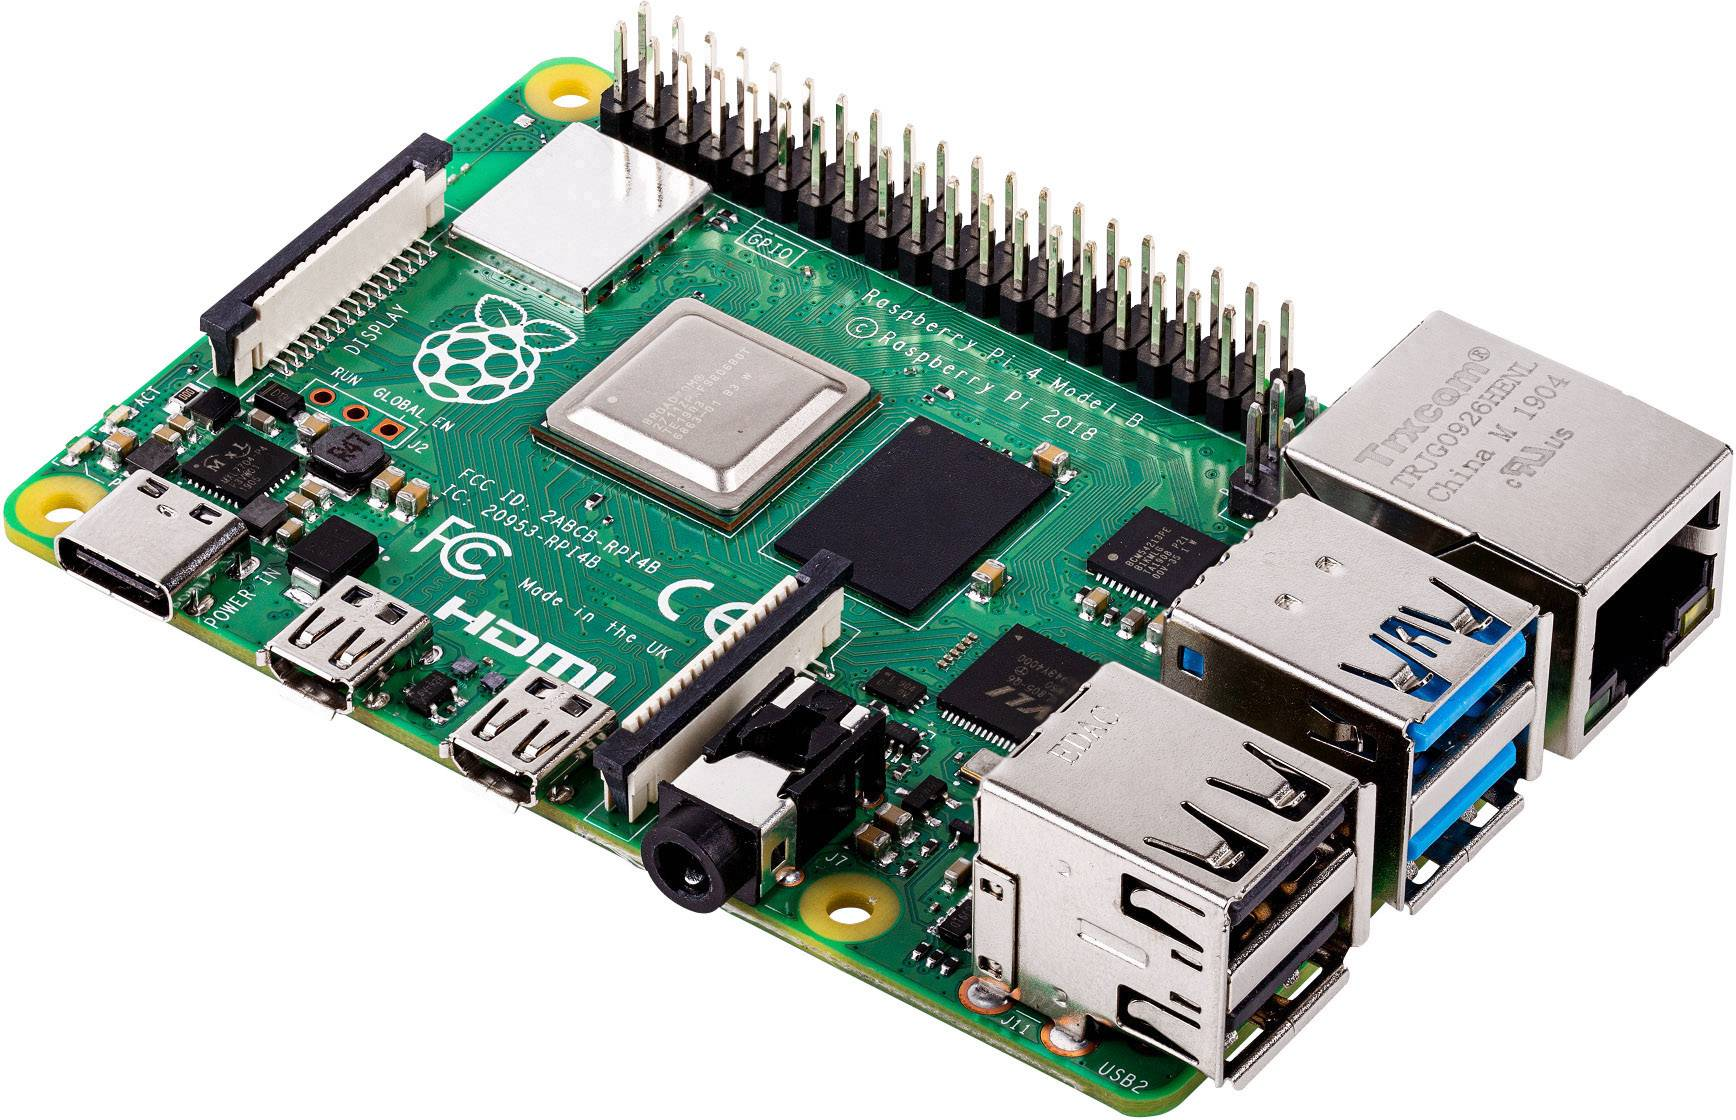
\includegraphics[width=\linewidth]{raspberryPi1}
    \caption{Raspberry Pi 4B}
    \label{fig:raspberry1}
\end{figure}

Een single board computer heeft een laag energiegebruik en de Raspberry Pi is geen uitzondering. Het heeft enkel een USB-C of microUSB kabel nodig voor stroom (afhankelijk van het model, zie figuur \ref{fig:raspberry2}). Deze zijn makkelijk te verkrijgen, aangezien de meeste smartphones dezelfde oplaadkabels gebruiken. Ook is de Raspberry Pi klein van formaat (85.6mm op 56.5mm). Dankzij dit formaat en het feit dat het weinig energie verbruikt, is er geen nood aan een ventilator om alle componenten koel te houden. Dus is de Pi uiterst stil, zelfs tijdens de grootste processen.(\cite{Foundationa}) 

\begin{figure}
    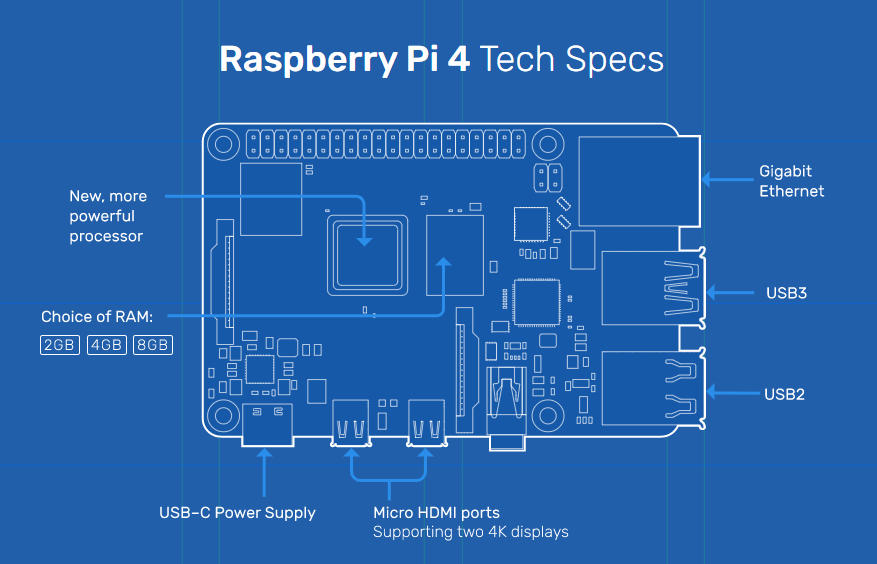
\includegraphics[width=\linewidth]{raspberryPiSpecs}
    \caption{Technische specificaties van de Raspberry Pi 4B}
    \label{fig:raspberry2}
\end{figure}

Tenslotte straalt de Pi uit op vlak van programmeertalen. Zo heeft de Pi zijn eigen besturingssysteem (zoals windows of IoS), genaamd Raspbian OS. Dit zorgt voor een makkelijke instap bij het gebruiken van de Pi. Ook komt het standaard met Python en Scratch: allebei makkelijk te gebruiken programmeertalen. Het hoeft echter daar niet te eindigen, aangezien het ook C++, C en Ruby geïnstalleerd heeft staan. Wanneer dit nog onvoldoende is, kunt u verschillende andere programmeertalen online installeren. Zo ondersteunt de Raspberry Pi zelfs Android applicaties. De Raspberry Pi Foundation heeft zelfs eigen cursussen en kits om de gebruiker te helpen bij elke stap van het programmeer proces \footnote{\url{https://www.raspberrypi.org/learn/}}.(\cite{Pattichis2017,Teja2021,Koelling2016})

Dankzij al deze eigenschappen is de Raspberry Pi een enorm flexibele optie om te gebruiken in de klas. De Pi is wel niet perfect. Zo heeft het bepaalde moeilijkheden die eventueel een obstakel kunnen vormen bij het gebruik ervan in de les. 
De Pi is relatief goedkoop tegenover een klassieke laptop of desktop, maar is wat aan de duurdere kant in vergelijking met andere single board computers. Ook zijn er een beperkt aantal verkopers van de Raspberry Pi en kan je deze enkel online vinden. Je kan ze dus niet makkelijk vinden in een gewone electronicawinkel. 
De Raspberry Pi is ook geen kant en klare technologie: je hebt andere componenten zoals een toetsenbord, een SD-kaart voor interne opslag en een scherm nodig vooraleer je kunt starten met programmeren. Dit kan het prijskaartje flink doen stijgen.

Tenslotte moet je voor het optimale gebruik van de Pi vaak speciale packages downloaden en installeren, waardoor de instap bij het gebruik van de Pi groter is dan andere single board computers. Hierdoor is er dus wat voorbereidingswerk nodig bij het gebruik van een Pi.(\cite{Teja2021})

De Raspberry Pi is dus niet de perfecte single board computer. Het heeft een goede prijsklasse en geniet dankzij zijn naambekendheid en open-source software van een grote community van Pi enthousiasten. Hierdoor bestaan er al veel projecten die gebruik maken van de kleine computer. Toch, de nood aan externe toestellen zoals een scherm en een toetsenbord is niet alleen onpraktisch, maar ook prijzig. Het heeft ook concurrentie die stilaan aan bekendheid wint en vaak goedkopere alternatieven biedt, zoals de Arduino. Ook is de Raspberry Pi en andere single board computers nog niet bekend in het onderwijs en zijn leerkrachten over heel de wereld nog sceptisch over deze kleine computers. Er is dus nog ruimte voor een alternatieve single board computer.(\cite{Susan2014})

\subsection{Arduino}

Arduino, opgericht in 2005 in Ivrea (Italië), is bekend voor het maken van de Arduino lijn van microcontrollers. Een microcontroller is een apparaat met een geïntegreerde schakeling (IC) die wordt gebruikt om andere delen van een elektronisch systeem te besturen. Een Arduino kan dus gebruikt worden om een bepaalde input om te vormen naar een nieuwe output (zie figuur \ref{fig:arduino1}). De oprichters van Arduino zochten een oplossing om snel en makkelijk verschillende elektronische componenten, zoals sensoren en motoren, aan elkaar te koppelen via hardware en software. Dit moest ook goedkoop blijven om niemand te limiteren in hun creativiteit. Met die gedachtegang werd de Arduino een waanzinnig succes zowel bij artiesten\footnote{een voorbeeld van een kunstwerk, gemaakt met een Raspberry Pi: \url{https://www.raspberrypi.org/blog/interactive-origami-art-with-raspberry-pi/}} als in het onderwijs. (\cite{Hughes})


\begin{figure}
    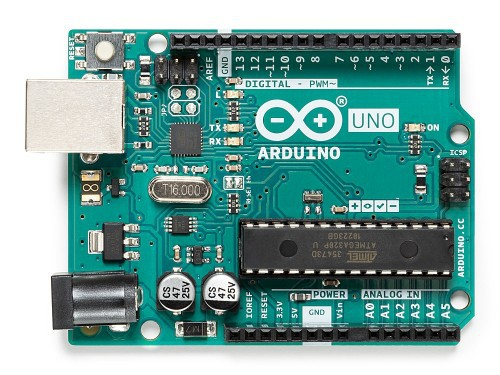
\includegraphics[width=\linewidth]{arduino}
    \caption{Arduino Uno Rev3}
    \label{fig:arduino1}
\end{figure}

De Arduino staat bekend voor zijn makkelijke instap. Met de plug-and-play eigenschap van de Arduino, kan men makkelijk sensoren verbinden met de arduino om zo een input te kunnen registreren. Dankzij de Arduino Integrated Development Environment (IDE) kan men makkelijk deze input omvormen naar een output die kan gestuurd worden naar een output apparaat zoals een motor of zelfs een andere Arduino. Voor de duidelijkheid: een Integrated Development Environment is software die een gebruiker de mogelijkheid geeft om leesbare code te schrijven. Je kan met een Arduino zowel programmeren met de Arduino programmeertaal\footnote{Een variant van C++} als met C of C++. Je kan zelfs andere programmeertalen downloaden.(\cite{Teja2021})

Nog een punt vóór Arduino is zijn beginners vriendelijkheid. Niet alleen omdat de instap kleiner is, maar omdat de Arduino meer bestand is tegen eventuele incidenten. Zoals zijn plug-and-play eigenschap insinueert, kan je makkelijk de stroomkabel verwijderen zonder enige problemen of corruptie aan de bestanden. Alle lopende processen worden namelijk eerst afgesloten voor het apparaat compleet stroom verliest. De Raspberry Pi heeft niet zo’n functie en is dus gevoeliger voor corrupte bestanden bij stroomverlies. Daarnaast zijn zowel de Pi als de Arduino energiezuinig, maar ook hier blinkt de Arduino meer uit.(\cite{Teja2021})

Arduino heeft verschillende prijsklassen. Zijn bekendste model, de Arduino uno, heeft slechts een aankoopprijs van 20 euro. Ook heeft het verschillende starter kits speciaal ontworpen voor educationele toepassingen. Hierdoor staat de Arduino momenteel op de eerste plaats voor de meest geschikte microcontroller van dit onderzoek.

Dus de uitkomst is duidelijk: de Arduino wint het van de Raspberry Pi. Met zijn goedkopere aankoopprijs, kant en klare educationele kits en stroomverlies veiligheid lijkt dit de beste single board computer voor in de les toch? Spijtig genoeg voor de Arduino is dit niet het geval. 

Zoals eerder vermeld is de Arduino eigenlijk geen single board computer, maar een microcontroller. Een belangrijk aspect van de Arduino is het transformeren van input naar output door het gebruik van sensoren, maar deze 'hardware' kan enkel één applicatie tegelijk draaien. Het beschikt ook niet over een besturingssysteem. Tenslotte mist de Arduino bepaalde eigenschappen die nodig zijn om het een single board computer te noemen, zoals USB-poorten, hdmi-ingangen, ethernet slots en eventuele wifi receivers.

Vaak worden de Pi en de Arduino vergeleken omdat ze op het eerste zicht dezelfde taken uitvoeren. Het verschil ligt in het feit dat de Pi veel complexere en meerdere applicaties kan draaien juist omdat niet alles geïntegreerd is op één chip. Omdat de Arduino enkel een microcontroller bevat waarvan zowel de RAM als de opslag als de processor geïntegreerd staan op één chip, verliest het de optie om verschillende programma’s tegelijk te draaien.(\cite{Teja2021,Keim2019,FreeCodeCamp2017})

De Arduino valt in dit onderzoek dus uit, aangezien het geen single board computer is. Dit betekent wel nog niet dat de Raspberry Pi de beste optie is voor dit onderzoek. Daarvoor hebben we nog één ander voorbeeld van een single board computer die toch een goede concurrent kan vormen voor de Pi. 


\subsection{Micro:bit }
De Micro:bit (zie figuur \ref{fig:microbit1}), gesponserd door de BBC in Groot-Brittannië, is een leuk stukje tech volledig ontworpen om kinderen en jongeren te leren programmeren. Het is een printplaat met verschillende ingebouwde sensoren. De Micro bit ondersteunt zowel Python als Scratch en Microsoft MakeCode. Dankzij deze verschillende codeertalen kan deze input omgevormd worden naar een concrete actie op de Micro Bit zelf. Zo zijn er bijvoorbeeld een aantal led-lichtjes op de printplaat gemonteerd, om directe feedback te tonen aan de gebruiker. (\cite{Stager2018})


\begin{figure}
    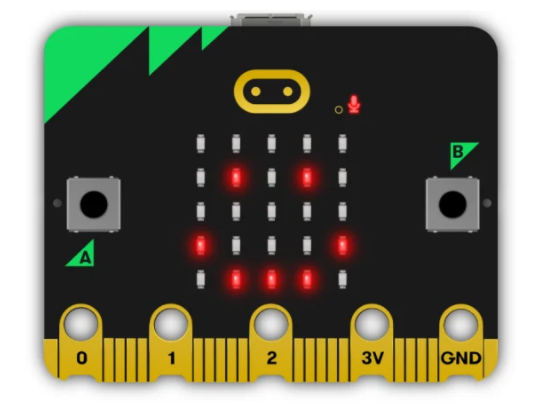
\includegraphics[width=\linewidth]{microbit}
    \caption{Micro:bit}
    \label{fig:microbit1}
\end{figure}

De Micro:bit heeft zoals de vorige, opgesomde voorbeelden een lage energieconsumptie. Wat de Micro:bit zo uniek maakt, zijn de verschillende power opties om de kleine techboard aan de praat te krijgen (zie figuur \ref{fig:microbit2}). Je kan op de klassieke manier een USB-port gebruiken voor stroom, maar ook een battery pack of via de 3V connectoren langs de rand van het toestel. Dit zorgt voor veel flexibiliteit en mobiliteit, iets wat niet kan gezegd worden van de PI.
Dit vernuftig stukje tech beschikt niet enkel over een usb-c connector en wat led-lichtjes. Het heeft een touch-sensor, speaker, radio antenne, 2 analoge knoppen en een microfoon. Hierdoor bespaar je toch wat geld bij het aankopen van sensoren. (\cite{Stager2018})

\begin{figure}
    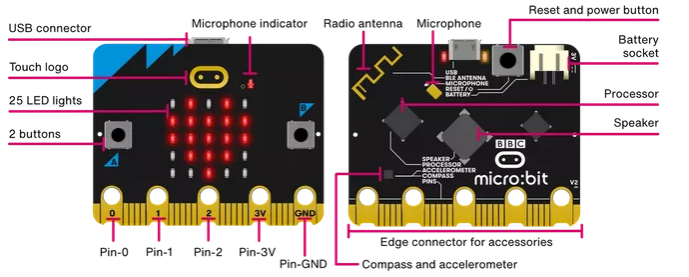
\includegraphics[width=\linewidth]{microbitSpecs}
    \caption{Technische specificaties van de Micro:bit}
    \label{fig:microbit2}
\end{figure}

Net zoals de Pi en de Arduino, heeft de Micro:bit een lage aankoopprijs. Zo koop je een Micro:bit GO v2 voor slechts 37,50 euro\footnote{\url{https://www.bol.com/nl/p/microbit-go-v2/9300000019150594/?bltgh=m-pQlfTCD-xYiTss1eNGrA.2_34.36.ProductTitle}}. Dit geeft de Micro:bit een edge boven de Raspberry Pi, die moeilijker online verkrijgbaar is. De Micro:bit heeft ook een intern geheugen, dus is er geen nood aan het kopen van een SD-kaart als geheugen. Hierdoor heeft de Micro:bit een soortgelijke plug-and-play eigenschap van die de Arduino ook bezit.

Tenslotte, juist omdat het doel van de Micro bit exclusief gericht is op educatie, heeft de Micro:bit een grote bibliotheek aan lessen en projecten. Deze zijn makkelijk te vinden o.a. op de  website van Micro:bit zelf\footnote{\url{https://microbit.org/}}. Hierdoor is het makkelijk voor een leerkracht om zo’n project te implementeren in zijn of haar lessen. Opnieuw een plus punt voor de Micro Bit.

In Groot-Brittannië is er zelfs onderzoek gedaan naar het gebruik van de Microbit om te leren programmeren. Zo hebben alle kinderen van het eerste jaar secundair onderwijs gratis een Micro:bit ontvangen die ze konden gebruiken in de les. Na het onderzoek bleek dat 90 procent van de jongeren een eigen project kon coderen en 88 procent leerde dat coderen niet zo moeilijk bleek te zijn. Zelfs meisjes, die door de stereotypen moeilijker te overhalen zijn om te leren programmeren, werd er een stijging in interesse vastgesteld met niet meer dan 70 procent. Ook leerkrachten ondervonden dat de Micro:bit een plezante en creatieve manier is om kinderen te leren programmeren. (\cite{IW2017})

Spijtig genoeg stoppen hier ook de voordelen van de Micro:bit. Het het grote nadeel waardoor het niet kan winnen van de Raspberry Pi: om te kunnen programmeren met een Micro:bit, heb je een externe computer nodig. Dit zorgt ervoor dat het argument van het prijskaartje volledig wegvalt. Ook kan men argumenteren dat om grafisch te leren programmeren, men geen nood heeft aan een Micro: bit, aangezien al het codeerwerk gebeurt op de externe computer.(\cite{Singapore})

Tenslotte is men niet zeker of de Micro Bit kan geclassificeerd worden als een single board computer. Sommige bronnen tonen aan van wel, aangezien het meer componenten bevat dan een Arduino, een typisch voorbeeld van een microcontroller. Andere bronnen beweren dat, door het feit dat het niet kwalificeert als een volledig geïntegreerde computer, het niet kan gezien worden als een single board computer. Meningen verschillen hierover. 
Na overleg met Francis Wyffels, professor in embedded systems aan de UGent, is er geconcludeerd dat de Micro:bit moeilijk in een categorie kan geplaatst worden. Het heeft zowel eigenschappen van een single board computer als van een microcontroller. Zo beschikt het over een krachtige ARM processor (eigen aan single board computers), maar heeft het ook alle nodige elementen zoals werkgeheugen ingebouwd in een enkele chip. (eigen aan een microcontroller). 

Toch poseert de Micro:bit zich als een groot concurrent van de Raspberry Pi. Met zijn grote catalogus aan vooraf opgestelde lessen en zijn leuke ingebouwde sensoren, lijkt de Micro:bit een geschikte optie om kinderen te leren grafisch programmeren. Vooral met programmeertalen zoals Scratch, lijkt deze single board computer een ideale oplossing voor ons onderzoek.Je kan ook makkelijk online een Micro:bit aankopen via Belgische e-shops zoals Bol.com. 

\subsection{Verdict}

Na het evalueren van deze drie opties blijkt slechts één single board computer het meest geschikt zijn voor het gebruik in een klasomgeving. Zo moet de single board computer niet alleen financieel voordelig zijn, maar moet er ook genoeg documentatie over bestaan om leerkrachten te helpen. Het moet kunnen beschikken over gemakkelijke programmeertalen en het moet voor beginners vriendelijk genoeg zijn, zonder creativiteit en flexibiliteit te limiteren.
Tenslotte zou de single board computer moeten kunnen opboksen tegen klassieke pc’s om deze te vervangen in de klaslokalen.

Rekening houdend met de beschreven criteria (zie figuur \ref{fig:swotsbc}) blijft uit de vergelijkende studie slechts één single board computer over: de Raspberry Pi. Het is de enigste volwaardige single board computer die werd opgenomen in dit onderzoek en is de enigste minicomputer die volledig zelfstandig kan werken. De Arduino is gebruiksvriendelijker dan de Raspberry Pi, maar is primitiever in zijn werking en is zelfs geen single board computer. De Micro:bit staat op een dichte tweede plaats. Aangezien de Micro:bit ontworpen is voor het gebruik in de klaslokalen lijkt het de ideale oplossing, maar door zijn nood aan een externe computer kan het moeilijk een klassieke computer vervangen als het op grafisch programmeren aankomt. Hoewel de Raspberry Pi een hogere instap nodig heeft dan voorgenoemde voorbeelden, vormt het de meest geschikte keuze voor dit onderzoek.


\begin{figure}
    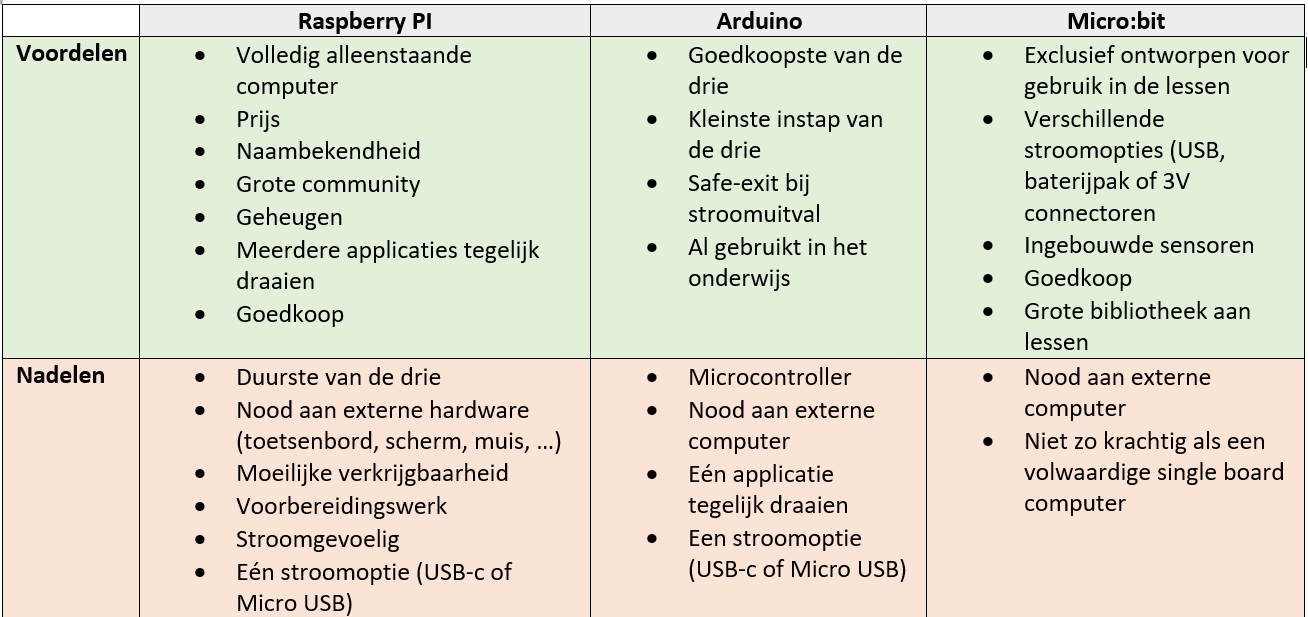
\includegraphics[width=\linewidth]{VoorEnNadelenSBC}
    \caption{SWOT-analyse van de single board computers}
    \label{fig:swotsbc}
\end{figure}

\section{Vergelijking van programmeertalen}

\subsection{Programmeertalen}

Na het bestuderen van de nodige eindtermen en competenties die men moet bereiken in de eerste graad secundair onderwijs en het uitkiezen van de meest geschikte single board computer als leertool, komt nu het moment om de meest geschikte programmeertaal te bepalen voor de proof of concept. Het kiezen van een juiste programmeertaal als starter taal is een belangrijke stap bij het leren programmeren. Zo kan een te moeilijke programmeertaal een gevoel van angst en frustratie opwekken tegenover coderen. Maar een te makkelijke taal kan snel saai worden voor de gebruiker. 

Eerst en vooral is het belangrijk om te begrijpen wat een programmeertaal inhoudt en welke soorten er momenteel bestaan. Zo is niet elke programmeertaal dezelfde en kan de complexiteit enorm verschillen. 
Een programmeertaal is een set opdrachten, instructies en andere syntaxis gebruiken om software te maken programma\footnote{\url{https://techlib.nl/definition/programming_language.html}}. Via een programmeertaal kan je communiceren met de hardware van een computer. Spijtig genoeg kan je niet zomaar instructies geven in het Nederlands en verwachten dat de computer het verstaat. De ingegeven taal moet vertaald worden naar een taal die de computer begrijpt. Een programmeertaal bestaat dus in essentie uit twee niveuas: 
\begin{itemize}
    \item Programmeertaal op hoog niveau
    \item Programmeertaal op laag niveau
\end{itemize}
 Een taal op hoog niveau is de taal waarin de programmeur programmeert. Deze taal moet voldoen aan een specifieke syntax. Deze taal is begrijpbaar, mits technische kennis. Hiermee kan de programmeur zich volledig focussen op het oplossen van problemen en hoeft hij zich niet zorgen te maken over technische zaken. 
  
 Je hebt ook talen op laag niveau. Dit is de taal die computers kunnen lezen en die onleesbaar is voor de mens. Deze taal bestaat vooral uit enen en nullen die we binaire code noemen. De computer kan de geschreven code van de programmeur niet lezen. Dus moet de geschreven code vertaald worden naar een taal op laag niveau.

Programmeertalen komen voor in verschillende soorten. Deze kunnen variëren van structuur tot architectuur. In het belang van dit onderzoek moet men het onderscheid begrijpen tussen text-based programmeertalen en block-based programmeertalen. Men vindt beide terug in een educatieve settings.

Text-based programmeren is de traditionele vorm van programmeren. Hierbij typt de gebruiker lijntjes code uit in een Integrated Development Environment, of kortweg IDE. Een IDE is simpelweg een omgeving om leesbare code te schrijven\footnote{\url{https://www.transip.be/knowledgebase/artikel/3305-wat-is-een-ide/?utm_source=knowledge}}. Je kan bijvoorbeeld geen leesbare code schrijven in Microsoft Word, maar wel in een IDE zoals Visual Studio, Eclipse of Xcode. De lijntjes code worden in de IDE omgezet naar leesbare code voor de computer.

Een voordeel van text-based programmeren is dat bijna alle professionele programmeertalen text-based zijn. Als je dus leert programmeren met een text-based programmeertaal, kan je makkelijker andere talen begrijpen en implementeren. Een groot nadeel is dat er een bepaalde syntax- en codeer-kennis nodig is om deze optimaal te kunnen gebruiken. De instap is dus groter. 

Block-based programmeren is een nieuwere manier van programmeren en is een stuk gebruiksvriendelijker. Block-based gebruikt het “programming-primitive-as-puzzle-piece” metafoor om programmeren op een meer visuele manier voor te stellen. Zo worden instructies voorgesteld als puzzelstukjes die men in een bepaalde volgorde kan slepen. Naargelang de lengte van het aantal puzzelstukjes en de complexiteit van de instructies kan men op een gemakkelijke en creatieve manier grote taken opsplitsen. Dit is een praktische uitwerking van computationeel denken. De lage complexiteit en het visuele aspect maakt van block-based programmeren een makkelijke eerste stap in de wereld van coderen. 

Een nadeel van block-based is dat het te abstract wordt afgebeeld in vergelijking met traditionele programmeertalen. Om professioneel te leren programmeren is men verplicht om de stap te maken van block-based naar text-based. Aangezien beide vormen zo hard verschillen, kan dit weleens een probleem vormen.(\cite{Weintrop2019,Maloney2010})

Nu deze belangrijke principes zijn opgeklaart kunnen we onze twee kandidaten voor de meest geschikte programmeertaal onderzoeken: Scratch en Python. Beide worden vaak gebruikt in een educationele context, maar zijn fundamenteel verschillend. 

\subsection{Scratch}

Scratch is een block-based programmeertaal. Ontworpen door de Scratch Foundation als non-profitorganisatie, is deze codetaal speciaal ontworpen om kinderen te leren programmeren, vanaf ongeveer acht jaar oud. Met Scratch kunnen kinderen en jongeren via de Scratch programmeertaal creatieve projecten uitbouwen zoals animaties, muziek en zelfs games. De software is volledig gratis om te gebruiken, dus iedereen kan er mee aan de slag. Scratch straalt uit in zijn gemakkelijk te gebruiken IDE en zijn beginners vriendelijke manier van werken.(\cite{Weintrop2019,Maloney2010})

Zoals vermeld is Scratch block-based: instructies worden voorgesteld als puzzelstukken die men in elkaar kan klikken om acties uit te voeren op het presenteer scherm. Zo is de UI van Scratch opgedeeld in een drie delen (zie figuur \ref{fig:scratch2}):
\begin{itemize}
    \item componenten paneel
    \item ontwerp paneel
    \item presentatiepaneel
\end{itemize}

\begin{figure}
    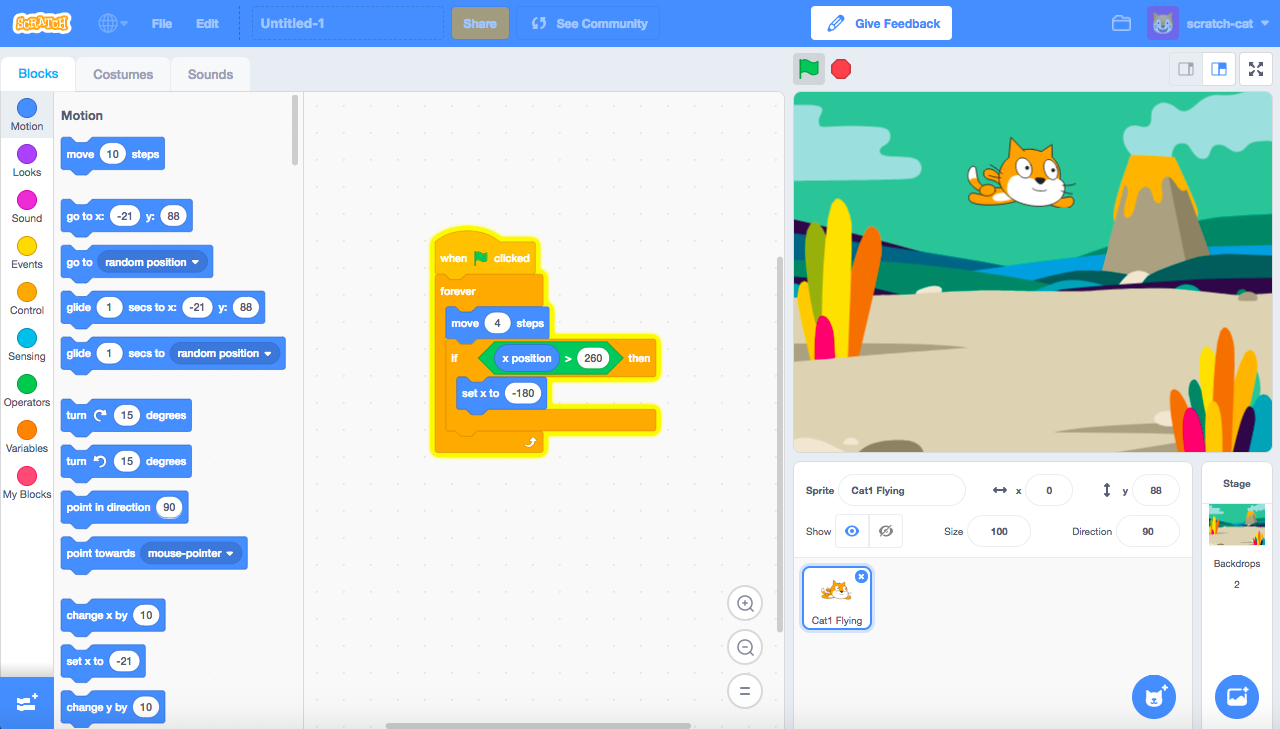
\includegraphics[width=\linewidth]{scratchIDE}
    \caption{Scratch}
    \label{fig:scratch2}
\end{figure}

Men sleept de nodige puzzelstukken of componenten van het componenten paneel naar het ontwerp paneel om instructies te koppelen aan elkaar. De componenten met de instructies erin worden aan mekaar gelinkt om acties te kunnen uitvoeren op het presentatiepaneel. Hier worden de instructies gevisualiseerd aan de hand van figuren en props. Zo kan men bijvoorbeeld een mannetje van links naar rechts laten bewegen op het presentatiepaneel door verschillende combinaties te maken in het ontwerp paneel. (\cite{Maloney2010})

Het geheel vormt een intuïtieve manier om computationeel denken te kunnen illustreren. Dankzij \textbf{decompositie} wordt een taak zoals het verplaatsen van een figuurtje opgedeeld in kleinere puzzelstukken. Via \textbf{abstractie} worden die puzzelstukken niet te complex voorgesteld en is de taak van een enkele puzzelstuk duidelijk. Met \textbf{patroonherkenning} kan men eventueel nagaan of men dezelfde code ook kan gebruiken om het figuurtje op en neer te laten bewegen. Daarna worden alle puzzelstukken aan elkaar gelinkt in een visueel \textbf{algoritme}. (\cite{Maloney2010, Weintrop2019})

Scratch helpt jongeren ook bij het voorkomen van foutieve links. Zo worden puzzelstukken die een foutboodschap kunnen generen wanneer gelinkt uitgesloten. Deze puzzelstukken kan je dus niet verbinden. Zo leren jongeren ook de kleine problemen kennen die deel uitmaken van het coderen.(\cite{Maloney2010})

Dankzij de website van Scratch\footnote{\url{https://scratch.mit.edu/}} kan men makkelijk oefeningen geschikt voor de klas vinden. Er bestaan ook veel externe projecten dankzij de naambekendheid van Scratch zelf. Zo maakt de Vlaamse organisatie CodeFever\footnote{Een onderneming die programmeerlessen organiseert voor kinderen in hun vrijetijd. \url{https://www.codefever.be/nl}} gebruik van het Scratch platform om kinderen en jongeren in hun vrije tijd te leren programmeren. Scratch wordt gezien als een ideale eerste stap in het leren coderen.

Er zijn wel wat nadelen verbonden bij het gebruik van Scratch. Zoals eerder vermeld komt de beginners vriendelijkheid van block-based programmeren met een kost. Scratch is hier geen uitzondering op. Hoewel Scratch de basisfundamenten illustreert van programmeren, is het geen professionele codetaal. Scratch is enkel een leermiddel en wordt niet gebruikt in de professionele wereld. Hierdoor kan je met enkel Scratch kennis niet verder leren programmeren. Je zal zelf de stap moeten maken naar text-based programmeren.
Ook kan de nogal kinderlijke manier waarmee Scratch code presenteert minder interessant lijken voor een tiener publiek. Ook jongeren die al meer kennen van programmeren kunnen gedemotiveerd raken door de simpliciteit. In een onderzoek over het leren met Scratch vroegen sommige leerlingen zich af of dit kon bekeken worden als “authentiek programmeren”. 
Tenslotte kan de simpliciteit limiterend werken. Omdat code kant en klaar voor de gebruiker wordt geschreven, is er weinig plaats om zelf te experimenteren met code. (\cite{Armoni2015,Fagan2017})

Scratch is een solide basis om te leren computationeel denken en programmeren. Zijn ludieke manier van programmeren kan jongeren helpen de interesse te kweken om verder te leren programmeren. Maar door zijn simpliciteit en door zijn beperkingen kan dit ironisch genoeg creativiteit limiteren. Gelukkig voor dit onderzoek hebben we nog een tweede optie: Python

\subsection{Python}

Python is een klassieke text-based programmeertaal. De gebruiker schrijft zelf de instructies uit die de computer moet uitvoeren. Dit, in tegenstelling tot een grafische programmeertaal zoals Scratch, is de meest gebruikte vorm van programmeren en is de norm in de professionele wereld. Python is een open-source codetaal: iedereen mag er gratis gebruik van maken, zonder te betalen. Dit is niet zo abnormaal in de wereld van codetalen: heel wat programmeertalen zijn open-source. Wat Python uniek maak, is zijn lage complexiteit. In tegenstelling tot bekende programmeertalen zoals Java, is gemakkelijk te lezen en is de instap veel lager. 


Python is wat ze noemen een “interpreted language”. Dit betekent dat de code niet eerst moet gecompileerd worden voordat men de code kan starten. Bij compilatie zal de interpeter lijn per lijn de taal op hoog niveau integraal omzetten naar een laag niveau. Hiermee is het makkelijker om een fout op te sporen in de code, aangezien de code stopt op de lijn waar de fout gevonden is. (\cite{Karani2020})

In tegenstelling tot Scratch is Python niet enkel gelimiteerd tot een learning tool: Python wordt zowel gebruikt in educationele applicaties als in professionele projecten. Dankzij de flexibiliteit van text-based is er meer vrijheid om nieuwe ideeën te proberen. Je bent niet gelimiteerd aan voorgemaakte puzzelstukken. Zo kan men ook low-level problemen leren aanpakken die bij block-based genegeerd worden. Ook kan men makkelijker andere text-based programmeertalen leren in vergelijking met block-based programmeren.

Vervolgens, dankzij zijn open-source eigenschap, bestaat er een grote actieve community van Python enthousiasten met een grote catalogus aan projecten. Deze kunnen reiken van simpele applicaties tot uitgebreide artificiële intelligenties\footnote{\url{https://www.edureka.co/blog/artificial-intelligence-with-python/}}. Dankzij de diversiteit aan Python projecten is er voor elk wat wils. Zo kunnen de beginnende leerlingen makkelijke opdrachten uitvoeren terwijl ervaren jongeren grotere uitdagingen kunnen tackelen. 

Tenslotte bestaan er veel voorgeprogrammeerde pakketten die men makkelijk kan importeren in de IDE om tijd te besparen. Hierdoor kan een leerling sneller aan de slag en hoeft hij niet perse alles zelf uit te typen. Dankzij zijn open-source eigenschap is er ook een grote catalogus van pakketten om uit te kiezen.

Hoewel Python een betere voorbereiding is op “echt programmeren”, heeft het zelf ook wat nadelen. Om te beginnen is de instap bij text-based programmeren een stuk groter dan bij block-based. Men heeft een bepaalde voorkennis nodig vooraleer men aan de slag kan. Dit maakt het lastiger voor leerkrachten om dit te organiseren in een klas.
In de eerste graad is het vooral belangrijk dat leerlingen de onderdelen van computationeel denken kunnen toepassen. Om Python te gebruiken moeten ze daarboven op ook de syntax eigen maken. De stap van probleem tot applicatie wordt dus groter. 
Er is ook een bepaalde taalbarrière bij text-based programmeren: de syntax van Python leunt aan bij het engels. Op zich zou dit geen probleem vormen, maar dit kan een obstakel vormen bij bepaalde leerlingen die minder goed zijn in die specifieke taal.
Tenslotte, juist omdat het een “interpreted language” is,  is Python een stuk trager in het uitvoeren van code. Omdat de vertaling van hoog niveau naar laag niveau pas gebeurt bij het uitvoeren van code, duurt het langer om een resultaat te zien.(\cite{Armoni2015})

Python is een klassieke programmeertaal, maar staat bekend voor zijn lage complexiteit en grote ondersteuning. Toch is er een bepaalde voorkennis nodig en is het organiseren van lessen met Python iets minder vanzelfsprekend als bij Scratch.

\subsection{Verdict}

Beide voorgestelde programmeertalen hebben hun unieke kwaliteiten. Scratch is enorm gebruiksvriendelijk en is gemaakt als leermiddel. Python is flexibeler in het maken van applicaties en heeft een groter toekomstbeeld. Ook hebben beide hun problemen: Scratch kan zeer simplistisch zijn en Python kan te complex zijn voor beginnende leerlingen. 

In de aard van dit onderzoek is er echter één programmeertaal die aan de meeste criteria voldoet: Python. Hoewel de instap moeilijker zal zijn bij Python, kan je meer bijleren als je zelf je code moet schrijven in tegenstelling tot voorgekauwde componenten. Met Python leer je elk deel van programmeren kennen, ook het falen. Juist omdat Scratch zo simpel is, negeert het vaak low-level, essentiële aspecten zoals het opvangen van fouten. 

Uit onderzoek van Armony Meerbaum-Salant en Ben-Ari blijkt dat leerlingen die met Scratch werken sneller vaardigheden kunnen leren van computationeel denken, maar dat na verloop van tijd het voordeel van de simpliciteit wegvalt. Met Python leren de studenten iets trager programmeren, maar halen ze na een periode van tijd dezelfde resultaten als de Scratch groep. Hieruit komt dan de vraag of het voordelig is om leerlingen eerst tijd te laten spenderen in het leren van Scratch om dan later toch over te schakelen naar text-based programmeertalen. (\cite{Armoni2015,Fagan2017})

Zelfs de taalbarrière vormt een minder groot probleem, aangezien uit onderzoek bewezen is dat het niveau Engels van vlaamse kinderen al gemiddeld hoger ligt dan vroeger. Er zijn dus weinig redenen om Scratch boven Python te kiezen. (\cite{Denies2015})




